\begin{history}

    In diesen Jahren durchlebte die Musikgesellschaft Hildisrieden eine
    spannende und dynamische Periode, die durch musikalische Erfolge,
    gesellschaftliches Engagement und wichtige Entwicklungen gekennzeichnet war.
    Unter der Führung der Dirigenten Franz Limacher, Thomas Zemp, Marcel
    Sennhauser, Beatrice Renkewitz und zuletzt Kobi Banz, erlebte der Verein
    eine stetige musikalische Evolution und festigte seine Rolle im kulturellen
    Leben von Hildisrieden. Die Musikgesellschaft engagierte sich regelmässig
    bei lokalen kirchlichen Anlässen wie Weisssonntag, Fronleichnam und
    Firmungen, am Zunftbot und Fasnachtsumzügen und vielen weiteren Anlässen im
    Dorf.

    Die jährlichen Konzerte der Musikgesellschaft, ergänzt durch spezielle
    Events wie Kirchenkonzerte, Auftritte im Shopping Center Emmen oder beim
    Pavillon in Luzern, bildeten das musikalische Fundament des Vereins. Darüber
    hinaus waren die Teilnahmen an kantonalen und eidgenössischen Musikfesten
    Highlights, bei denen die Musikgesellschaft ihr musikalisches Talent und
    Können sowohl in konzertanten Darbietungen als auch in der Marschmusik
    demonstrierte. Trotz gelegentlicher Herausforderungen und Enttäuschungen
    über Wettbewerbsbewertungen blieb der Verein leidenschaftlich und
    zielorientiert.

    Ein besonders prägendes Ereignis war die Fahnenweihe im Jahr 1984, die nicht
    nur die Verbundenheit der Musikgesellschaft mit ihren Traditionen zeigte,
    sondern auch den Gemeinschaftssinn und Stolz auf das gemeinsame Erbe zum
    Ausdruck brachte.

    Die Neuuniformierung neun Jahre später, im Jahr 1993, stellte einen weiteren
    bedeutenden Meilenstein dar. Sie symbolisierte Erneuerung und Fortschritt
    und bekräftigte die visuelle und kulturelle Identität des Vereins in der
    Öffentlichkeit. Dieses Ereignis wurde mit einem festlichen Wochenende
    zelebriert, einschliesslich eines Galakonzerts der Brassband Bürgermusik
    Luzern, und stärkte das Gemeinschaftsgefühl innerhalb von Hildisrieden.

    Zusätzlich zu diesen musikalischen und kulturellen Aktivitäten engagierte
    sich die Musikgesellschaft in der musikalischen Förderung des Nachwuchses
    und in Kooperationen mit anderen Musikvereinen. Sie organisierte
    Instrumentenparcours und unterstützte musikalische Bildungsinitiativen.

    Soziale Veranstaltungen, Ausflüge und gemeinschaftliche Feste förderten den
    Zusammenhalt und die Kameradschaft innerhalb der Musikgesellschaft. Von
    Chilbis über Waldfeste bis hin zu Lottoabenden - diese geselligen Anlässe
    trugen nicht nur zur Finanzierung des Vereins bei, sondern auch zum
    lebendigen Vereinsleben und zur Stärkung der Gemeinschaft. Durch all diese
    Aktivitäten und Ereignisse zeigte die Musikgesellschaft Hildisrieden über
    zwei Jahrzehnte hinweg eine beeindruckende Vielfalt an Engagement und
    Leistung, was ihren unverzichtbaren Beitrag zum kulturellen und
    gesellschaftlichen Leben der Gemeinde Hildisrieden unterstreicht.

    \clearpage

    \subsubsection*{Kantonales Musikfest 1976 in Sempach}

    Im Vorfeld des kantonalen Musikfestes in Sempach am 24. Mai 1975 nutzten wir
    die Gelegenheit, unser Können durch eine Expertise von André Winkler
    schärfen zu lassen. In der Turnhalle wies er uns mit präzisen Kommentaren
    auf die Schwachstellen in unseren Stücken „nostalgische Ouvertüre“ und
    „Ouverture Symphonique“ hin. Am 13. und 14. Juni präsentierten wir diese
    Stücke abwechselnd mit der Musikgesellschaft Römerswil in einer
    eindrucksvollen Darbietung im Löwen und in der Kirche.

    Der Höhepunkt, das kantonale Musikfest in Sempach am 22. Juni, zeigte unsere
    musikalischen Bemühungen. Für die „Nostalgische Ouvertüre“ erhielten wir
    lobende 153 von 180 Punkten und für die „Ouverture Symphonique“, gespielt in
    der Kirche, sogar 160 Punkte. Diese Leistung brachte uns stolze 313 Punkte
    gesamt ein, womit wir den 5. Rang in der zweiten Stärkeklasse erreichten.
    Trotz einer etwas enttäuschenden Bewertung in der Marschmusik mit nur 29
    Punkten, endete der Tag auf eine hoch positive Note. Die Götschizunft und
    die Dorfbevölkerung bereiteten uns einen herzlichen Empfang, bei dem wir uns
    über die Unterhaltung durch die Trachtengruppe und den Kirchenchor freuen
    durften.

    \subsubsection*{Früher Verlust von Musikkameraden}
    In einer Reihe von tiefgreifenden Verlusten musste unsere Musikgesellschaft
    innerhalb kurzer Zeit von drei geschätzten Vereinskameraden Abschied nehmen.
    Der erste Abschied ereignete sich am 2. November 1978, als wir unseren
    Musikkameraden und Vicedirektor Marcel Stierli, der nur 32 Jahre alt wurde,
    zu Grabe trugen. Wir erwiesen ihm mit dem Ordonanzmarsch und dem Choral
    \enquote{Der gute Kamerad} die letzte Ehre.

    Wenige Monate später, am 12. April 1979, trauerten wir erneut, diesmal um
    unseren jungen Musikkameraden Erwin Luterbach, der im Alter von nur 21
    Jahren einem Arbeitsunfall zum Opfer fiel. Auch ihm gaben wir auf dem
    Friedhof das letzte Geleit.

    Ein weiterer schmerzlicher Verlust folgte am 11. Juni 1980, als unser
    Vereinskamerad Silvester Troxler im Alter von 56 Jahren von uns ging.

    Bei jedem dieser Abschiede standen wir zusammen, um unseren Freunden und
    Musikkameraden mit tiefer Verbundenheit und musikalischer Huldigung Respekt
    zu zollen und sie in Ehren zu halten.

    \subsubsection*{Eidgenössisches Musikfest 1981 in Lausanne}

    Die Teilnahme der Musikgesellschaft nach harter Probearbeit -- in 100 Tagen
    war der Verein 50-mal beisammen -- am eidgenössischen Musikfest 1981 in
    Lausanne war ein prägendes Ereignis, das allerdings nicht ohne
    Startschwierigkeiten begann.

    Schon auf der Hinfahrt nach Lausanne stiess die Reisegesellschaft auf ein
    unerwartetes Problem: Ein Reifen des Reisebusses verlor Luft, was zu einer
    unvorhergesehenen Verzögerung führte. Um das Problem zu beheben, musste der
    Bus in Rothenburg in eine Werkstatt gebracht werden, wo sich herausstellte,
    dass das Pumpen des Reifens schwieriger als gedacht war. Der Bus musste
    sogar mit einem Lift angehoben werden, um an den Reifen zu gelangen. Diese
    technischen Schwierigkeiten kosteten wertvolle Zeit, sodass das Gepäck und
    die Instrumente in einen Ersatzbus umgeladen werden mussten.

    Trotz dieser Startschwierigkeiten gelang es der Reisegruppe, mit einer
    Stunde Verspätung abzufahren und doch noch rechtzeitig in Lausanne
    anzukommen, um am Wettbewerb teilzunehmen.\\

    Tags darauf wurden Tonbandaufnahmen im Bauernschopf beim Rest. Schlacht
    aufgezeichnet.


    \subsubsection*{Solothurner Musikfest 1984 in Balsthal}

    Die Vorbereitung auf das Fest war von grosser Intensität geprägt -- nebst
    Expertisen wurde auch der Musiktag in Neuenkirch besucht -- die sich in
    einer engagierten Teilnahme und einem hervorragenden Abschneiden
    niederschlug.

    Die Musikgesellschaft trat mit den Stücken \enquote{Capriccio für Blasmusik}
    und \enquote{London River} an, wobei besonders die Darbietung des
    Selbstwahlstückes \enquote{London River} in der Kirche von der Jury mit
    hohen Punkten belohnt wurde.

    Diese Leistung führte zu einer Gesamtpunktzahl, die der Musikgesellschaft
    Hildisrieden einen überraschenden, aber wohlverdienten 1. Rang in der 3.
    Klasse einbrachte.

\end{history}

\groupphoto{0.93}{0.8}{./chap/1975-2000/1984/MGH-1984.jpg}
{\emph{Balstal 1984}\\
    1. Reihe:\\
    Portmann Toni, Gassmann Alois sen., Bucher Kandid, Disler Fritz, Estermann
    Hans, Zemp Thomas, Rüttimann Herbert, Troxler Hermann, Estermann Franz, Wolf
    Josef jun., Estermann Leo\\
    2. Reihe:\\
    Luterbach Walter, Rüttimann Franz, Troxler Pirmin, Estermann Alois,
    Estermann Anton, Fleischlin Anton, Dörig Franz, Käppeli Peter, Troxler
    Martin\\
    3. Reihe:\\
    Emmenegger Yvonne, Bachmann Anton, Estermann Othmar, Troxler Walter,
    Estermann Jakob, Koller Beat, Estermann Martin, Koller Alois\\
    4. Reihe:\\
    Wolf Josef sen., Stöckli Hans, Suter Jakob, Estermann Hugo, Estermann Bruno,
    Arnold Franz, Schmid Armin, Dörig Kaspar, Gassmann Alois jun., Estermann
    Otto, Rüttimann Walter, Estermann Niklaus } {fig:mgh-1984}

\clearpage
\begin{history}

    \subsubsection*{Fahnenweihe 1984}

    Die Feierlichkeiten zur Fahnenweihe begannen am Freitagabend mit einem
    gemütlichen Beisammensein von Musikliebhabern und der Ortsbevölkerung, zu
    Ehren des Patenpaares Lisbeth Lang-Ruckli und Fritz Amrein. Trotz starker
    Sturmböen waren wir über die Anzahl der Besucher erfreut.

    Am Samstagabend sorgte das Tanzorchester Dreams, auch ungeachtet des
    regnerischen Wetters, für eine ausgelassene Stimmung, während die
    Musikantenbar vor Besuchern kaum noch Platz bot.

    \begin{MulticolFigure}
        \centering
        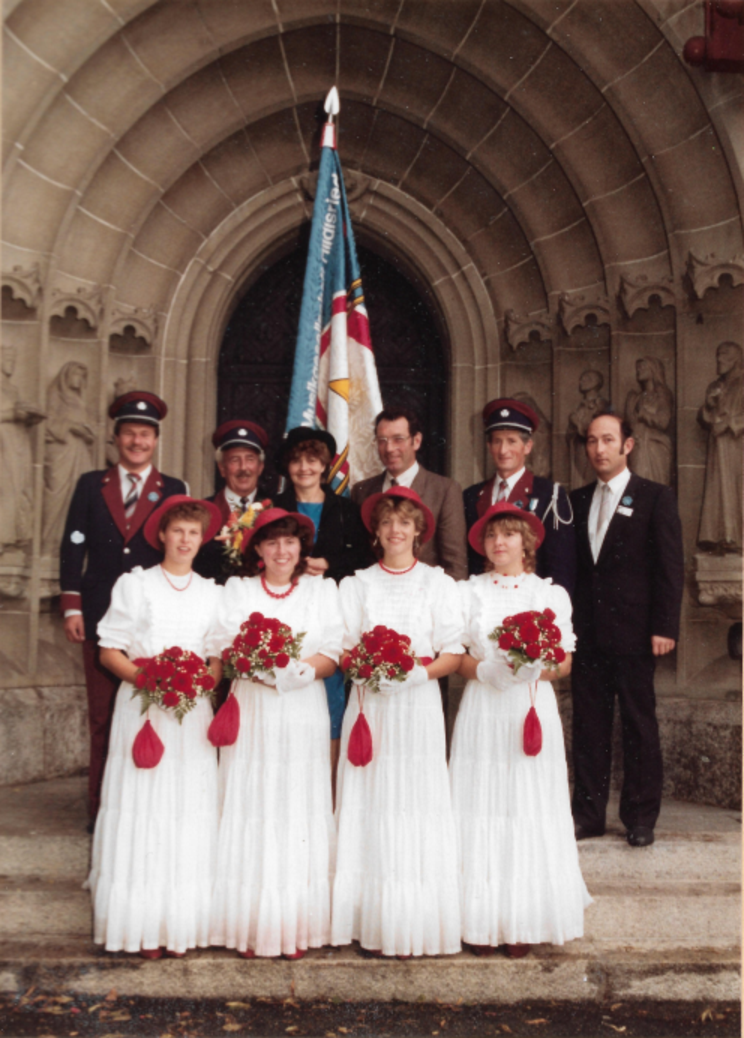
\includegraphics[width=0.6\linewidth]{./chap/1975-2000/1984/Fahnenweihe-1984.pdf}
    \end{MulticolFigure}

    Aufgrund des ungünstigen Wetters wurde die Fahnenweihe am Sonntag in die
    Kirche verlegt. Das musikalische Ständchen und der Aperitif im Anschluss an
    den Gottesdienst wurden rasch ins Festzelt umgezogen. Beim darauffolgenden
    Bankett waren mehrere bedeutende Persönlichkeiten zu Gast. Im weiteren
    Verlauf schlossen sich 17 Gruppen dem Festumzug an, nach dem sich Jung und
    Alt im Festzelt versammelten, um den Darbietungen benachbarter Musikvereine
    zu lauschen. Der OK-Präsident Walter Schmid hielt eine Rückschau auf die
    110-jährige Geschichte des Vereins.

    \multicolphoto{./chap/1975-2000/1984/MGH-Fahnenweihe-1984-Festakt.jpg}

    Den Abschluss am Dienstagabend gestalteten unsere lokalen Vereine und die
    Swiss Rolling Brass Band unter der Leitung von Franz Renggli, wobei Klaus
    Estermann als Moderator durch den Abend führte.

    \subsubsection*{Ausflug nach Lauterbach, Deutschland 1986}

    Vom 23. bis zum 25. Mai unternahm die Musikgesellschaft Hildisrieden eine
    dreitägige Reise nach Lauterbach, vermittelt durch den Einsatz ihres
    Dirigenten Thomas Zemp. Das Ziel war das malerische Städtchen Lauterbach,
    gelegen nahe Fulda und unweit der ehemaligen Grenze zur DDR, bekannt für
    seine gastfreundliche Atmosphäre und historische Bedeutung.

    Unter optimalen sommerlichen Wetterbedingungen startete die Gruppe ihre
    Reise in einem modernen Doppeldeckerbus. Nach einer Fahrt mit Zwischenhalten
    und der üblichen Verzögerung bei Stuttgart wurden die Ankömmlinge in
    Lauterbach herzlich empfangen. Die Unterbringung in Gastfamilien bot
    Gelegenheit zum direkten kulturellen Austausch und vertiefte das Erlebnis.

    Ein dichtes Programm erwartete uns am Samstag. Der Empfang durch den
    Bürgermeister und die musikalische Mitwirkung am traditionellen
    Prämienmarkt, trotz einsetzendem Regen, waren nur einige der Höhepunkte.
    Besonders eindrücklich war der Besuch an der Grenzschutzstation Hünfeld, wo
    die Reiseteilnehmer tiefe Einblicke in die Geschichte der deutschen Teilung
    erhielten.

    Die Abende wurden genutzt für musikalische Darbietungen und geselliges
    Beisammensein, bei dem die Musikgesellschaft ihr Können und ihre
    Vielseitigkeit unter Beweis stellte. Diese Momente des Austauschs und der
    Freude mündeten in langanhaltende Feierlichkeiten bis spät in die Nacht.

    Der Ausflug endete mit einem bewegenden Abschied, bei dem neu geknüpfte
    Freundschaften im Mittelpunkt standen.

    \subsubsection*{Unterwaldner Musikfest Sarnen 1987}

    Die finale Vorbereitung fand am 8. Mai mit einer Expertisenprobe unter der
    Leitung von Franz Renggli statt, um den musikalischen Ausdruck für das
    bevorstehende Fest zu verfeinern.

    Am 13. und 14. Juni präsentierte sich die Musikgesellschaft in Sarnen, wo
    sie zunächst mit dem Marsch \enquote{Diavolezza} auftrat, gefolgt von einer
    Darbietung der Ouvertüre \enquote{A Suite for Switzerland} von Roy Newsome
    in der Turnhalle. Die Aufregung und Spannung unter den Musikanten war gross,
    da die Ergebnisse erst am Tag nach dem Auftritt bekannt gegeben wurden, was
    zu Spekulationen und Hoffnungen innerhalb der Musikanten führte.

    Die abendliche Feier im Anschluss an das Bankett wurde zu einem denkwürdigen
    Teil des Festes, bei dem die Musikanten in der Linden in Sarnen ausgelassen
    feierten.

    Bei der Rangverkündigung am Sonntag stellte sich heraus, dass die
    Musikgesellschaft Hildisrieden den 20. Platz von 28 teilnehmenden Vereinen
    erreichte -- ein Resultat, das hinter den Erwartungen zurückblieb. Jedoch
    erzielte die MGH in der Marschmusik mit 90,5 Punkten einen hervorragenden 5.
    Rang.

    \subsubsection*{Reise ins Montafon 1988}

    Die Musikgesellschaft Hildisrieden begab sich am 27. und 28. August auf eine
    Musikreise ins Montafon, Österreich. Unter der Organisation von Toni
    Kleemann startete die Fahrt um 12 Uhr mittags mit einem Reisebus der Firma
    Estermann Beromünster und einem zusätzlich gemieteten Kleinbus. Die Route
    führte über Hirzel und den Walensee bis hin zum Fürstentum Liechtenstein, wo
    in Vaduz eine kurze Kaffeepause eingelegt wurde.

    Nach der Überquerung der Grenze und der Durchfahrt durch Feldkirch, Bludenz
    und Schruns erreichten wir schliesslich Partennen am Silvretta-Pass. Dort
    bezog man Quartier in drei gemütlichen Frühstückspensionen. Ein abendlicher
    Spaziergang bot Gelegenheit, das charmante Dorf und seine kulinarischen
    Angebote kennenzulernen. Der Höhepunkt des Abends war das gemeinsame
    Nachtessen im Unterhaltungskeller des Hotels Hubertusklause, wo der Wirt
    persönlich für musikalische Unterhaltung sorgte und für ausgelassene
    Stimmung unter dem Motto \enquote{Auf die Bäume ihr Affen, der Wald wird
        geputzt} sorgte.

    Der folgende Tag begann mit herrlichem Wetter, das zu weiteren Ausflügen
    einlud, sei es mit dem Bus zur Bielerhöhe oder zu Fuss zur Alp Tafamunt.
    Gegen Nachmittag hiess es dann, Abschied von der österreichischen
    Gastfreundschaft zu nehmen. Die Rückreise wurde mit einem überraschenden
    Zvieri in St. Gallenkappel bereichert, wo der ehemalige Musikkamerad Markus
    Dörig und seine Frau uns mit einem vorbereiteten Käsebuffet willkommen
    hiessen.

\end{history}

\groupphoto{0.93}{0.8}{./chap/1975-2000/1990/MGH-1990.jpg}
{\emph{Schüpfheim 1990}\\
    1. Reihe:\\
    Martin Estermann, Franz Estermann, Pirmin Troxler, Marcel Sennhauser, Josef
    Wolf jun., Franz Dörig, Leo Estermann, Alois Gassmann sen.\\
    2. Reihe:\\
    Anton Fleischlin, Hermann Troxler, Stephan Wolf, Armin Schmid, Otto
    Estermann, Kaspar Dörig, Jakob Suter, Bruno Estermann\\
    3. Reihe:\\
    Niklaus Estermann, Yvonne Emmenegger, Martin Gassmann, Albert Tschofen,
    Anton Bachmann, Anton Kleemann, Kaspar Troxler, Marcel Arnold, Walter
    Troxler\\
    4. Reihe:\\
    Beat Estermann, Andreas Krieger, Othmar Estermann, Peter Käppeli, Josef Wolf
    sen., Hans Stöckli, Walter Rüttimann, Alexander Troxler\\
    5. Reihe:\\
    Christoph Troxler, Kandid Bucher, Oskar Troxler, Hans Estermann, Franz
    Arnold, ???, Alois Gassmann jun. } {fig:mgh-1990}

\begin{history}
    \subsubsection*{Kant. Musikfest in Schüpfheim 1990}

    Die intensive Vorbereitungsphase, gekennzeichnet durch eine ganztägige
    Musikprobe im Lehrerseminar in Hitzkirch legte den Grundstein für eine
    solide Aufführung. Unter optimalen Bedingungen fokussierte sich die MGH auf
    die Feinheiten der beiden Wettkampfstücke, was die Basis für eine
    erfolgreiche Teilnahme bildete.

    Ein weiterer Schritt in der Vorbereitung war das Gemeinschaftskonzert am 5.
    Juni in der Festhalle Sempach, bei dem die Musikgesellschaft Hildisrieden
    zusammen mit den Musikgesellschaften Harmonie Sempach und Harmonie Rain die
    Wettkampfstücke präsentierte.

    Am 16. und 17. Juni fand schliesslich das kantonale Musikfest in Schüpfheim
    statt. Schon früh am Morgen begann wir mit den letzten Vorbereitungen und
    der Vorprobe. Trotz anfänglicher Nervosität gelang es, die Konzentration zu
    bewahren. Die Präsentation des Aufgabenstücks \enquote{Dies acterna} von
    Pascal Faver brachte der uns 159,5 Punkte ein, eine Bewertung, die gemischte
    Gefühle hervorrief, letztlich jedoch eine solide Leistung darstellte. Die
    Aufführung des Selbstwahlstücks \enquote{A Holiday Suite} von Eric Ball
    wurde von den Experten mit 168 Punkten belohnt, was die Musikgesellschaft
    Hildisrieden auf den ausgezeichneten 5. Rang katapultierte.

    Der Start zum Marsch \enquote{Hessen} gelang nicht ganz nach Wunsch, mit 41
    Punkten landeten wir im Mittelfeld. Nach der Rückkehr wurde die
    Musikgesellschaft von den Dorfvereinen herzlich empfangen.

\end{history}
\clearpage
\begin{history}

    \subsubsection*{Neuuniformierung und Teilinstrumentierung 1993}

    Über mehrere Tage hinweg feierte die MGH mit einer Vielzahl von
    Veranstaltungen.


    Die Feierlichkeiten wurden mit einem Galakonzert der Brassband Bürgermusik
    Luzern unter der Leitung von Ludwig Wicki eröffnet, das trotz frischen
    Wetters eine beeindruckende Menge an Blasmusikfreunden ins Festzelt lockte.
    Der Erfolg dieses Konzerts, zusammen mit dem beliebten Tessinerstübli, dem
    Café Symphonie, der Bar und der Bierschwemme, legte den Grundstein für die
    weiteren Festtage.

    Der darauffolgende Freitagabend war dem Dank an die Gönner der
    Musikgesellschaft gewidmet.

    \begin{MulticolFigure}
        \centering
        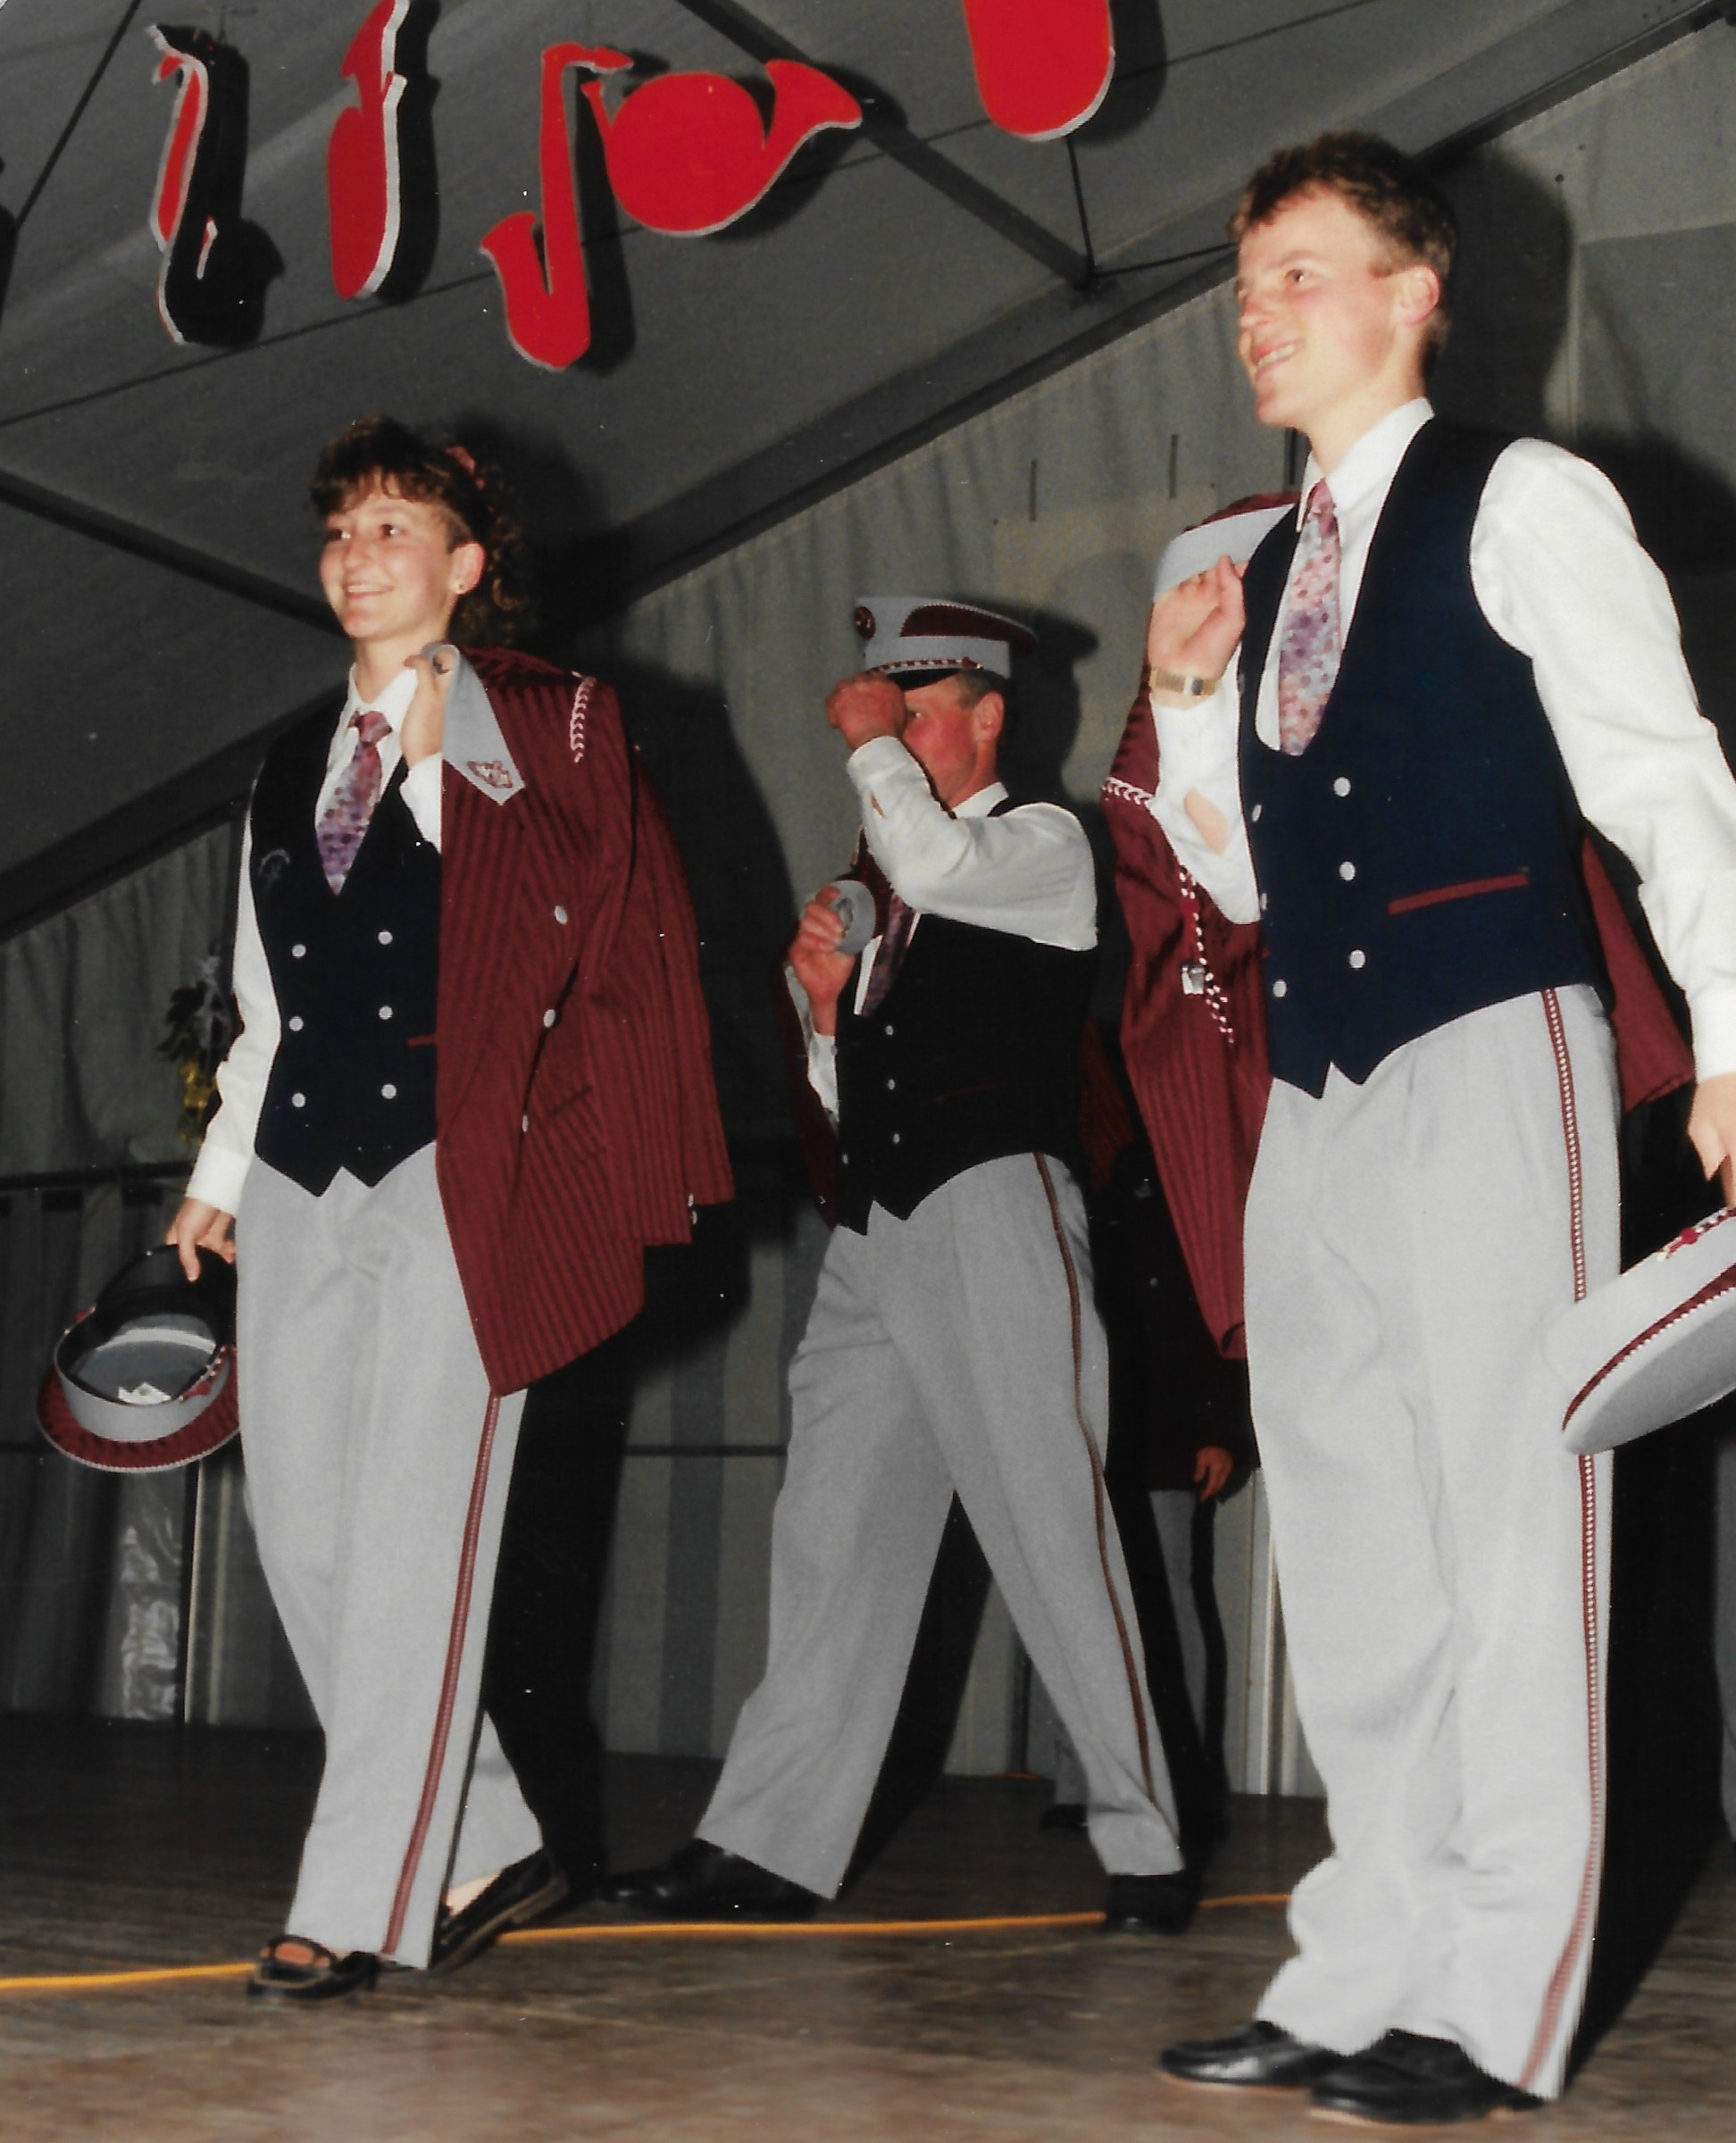
\includegraphics[width=0.55\linewidth]{./chap/1975-2000/1993/MGH-Vorstellung-Neue-Uniform-1993.jpg}
        \captionof{figure}{Die Models präsentieren die neue Uniform}
    \end{MulticolFigure}

    Ein Apéro und ein anschliessendes Abendessen im Festzelt dienten als Rahmen
    für die Präsentation der neuen Uniformen, was bei allen Anwesenden auf
    grosse Begeisterung stiess.

    Am Samstagabend war das Festzelt Schauplatz eines Tanzabends, der besonders
    die jüngere Generation anzog und die gesamte Nacht über gut besucht war. Die
    Beizli waren bis in die späten Stunden voll besetzt.

    \multicolphoto{./chap/1975-2000/1993/MGH-Neuuniformierung-1993-Totenehrung.jpg}

    Der Höhepunkt der Neuuniformierung fand am Sonntag statt, als die
    Musikgesellschaft erstmals in ihren neuen Uniformen auftrat.

    \multicolphoto{./chap/1975-2000/1993/MGH-Uniformweihe-1993-von-oben.jpg}

    Ein feierlicher Gottesdienst mit Uniformweihe durch Pfarrer Paolo Brenni und
    ein anschliessender Festumzug durch das Dorf, an dem auch die Harmonie Rain
    und zahlreiche Dorf- sowie Nachbarvereine teilnahmen, demonstrierten den
    Stolz und die Freude der Musikgesellschaft und der Gemeinde.

    \multicolphoto{./chap/1975-2000/1993/MGH-Neuuniformierung-1993}
    Der Festakt im Zelt wurde von kurzen Ansprachen und der Uraufführung des
    Marsches \enquote{Free of Fog} begleitet. Der Abend klang mit Jazzmusik der
    Lake City Stompers und der Versteigerung künstlerisch gestalteter Collagen
    aus alten Instrumenten aus.

\end{history}


\groupphoto{0.93}{0.8}{./chap/1975-2000/1993/MGH-1993.jpg}
{\emph{Neuuniformierung 1993}\\
    1. Reihe:\\
    Peter Käppeli, Walter Troxler, Hans Estermann, Oskar Troxler, Leo Galliker,
    Cyril Hofer, Yvonne Emmenegger\\
    2. Reihe:\\
    Leo Estermann, Franz Dörig, Stephan Wolf, Thomas Wolf, Marcel Sennhauser,
    Bruno Estermann, Josef Wolf jun., Thomas Dörig, Pirmin Troxler, Franz
    Estermann\\
    3. Reihe:\\
    Alois Gassmann sen., Werner Bucher, René Zurfluh, Albert Tschofen, Martin
    Gassmann, Anton Kleemann, Hermann Troxler, Anton Bachmann, Beat Bachmann,
    Armand Troxler, Kaspar Dörig, Jakob Suter, Armin Schmid, Martin Estermann\\
    4. Reihe:\\
    Beat Estermann, Beat Koller, Jakob Estermann, Christoph Troxler, Othmar
    Estermann, Franz Arnold, Hans Stöckli, Josef Wolf sen., Reto Rüttimann,
    Alois Gassmann jun. } {fig:mgh-1993}

\begin{history}

    \subsubsection*{Eidg. Musikfest Interlaken 1996}

    Die Musikgesellschaft Hildisrieden bereitete sich intensiv auf das
    eidgenössische Musikfest 1996 in Interlaken vor, mit zwei
    Gemeinschaftskonzerten als Teil der Vorbereitungen. Das erste Konzert fand
    am 5. Juni in Römerswil statt, zusammen mit der Brass Band MG Römerswil und
    der Harmonie Rain, gefolgt von einem zweiten Konzert am 6. Juni in Eich mit
    der Musikgesellschaft Eich und der Harmonie Sempach. Beide Konzerte stiessen
    auf grosses Interesse und wurden enthusiastisch aufgenommen, was uns positiv
    stimmte.

    Am 15. und 16. Juni nahm die Musikgesellschaft am eidgenössischen Musikfest
    in Interlaken teil, wo sie sich in einem letzten Einspielen im Löwen auf die
    bevorstehenden Aufführungen einstimmte. Nach einem Ständchen für die
    Firmlinge ging es nach Interlaken, wo das gute Wetter ein hervorragendes
    Festival ankündigte. Im Aareparksaal präsentierten wir das Aufgabenstück
    \enquote{Offside} von Christian Henking, das mit 138 Punkten bewertet wurde
    -- eine Bewertung, mit der man nur mässig zufrieden war. Die Aufführung des
    Selbstwahlstücks \enquote{A Saddleworth Festival Ouverture} von Goff
    Richards in der Kirche von Unterseen brachte jedoch mit 149 Punkten eine
    deutlich positivere Resonanz und platzierte die Musikgesellschaft mit einem
    Gesamtergebnis von 287 Punkten auf den 9. Rang unter 41 teilnehmenden
    Vereinen, ein Ergebnis, das die Erwartungen übertraf und zur Zufriedenheit
    führte.

    Auch in der Marschmusik wollte man einen guten Eindruck hinterlassen, was
    mit 107 Punkten und einem überraschenden 12. Rang von 41 ebenfalls gelang.
    Die erfolgreiche Teilnahme und die erzielten Ergebnisse wurden anschliessend
    bis in die Morgenstunden gefeiert.

    \subsubsection*{Ausflug nach Seefeld, Tirol 1997}

    Die Reise führte mit einem Car von Estermann Beromünster über St.
    Margrethen, Bregenz, Oberstaufen und Immenstatt, bevor die wir gegen Abend
    in Seefeld eintrafen. Nach dem Beziehen der Zimmer und einem gemeinsamen
    Abendessen erkundeten einige Mitglieder die malerische Stadt, während andere
    sich direkt in den gemütlichen Bräukeller begaben, wo die erste von mehreren
    feucht-fröhlichen Festen mit Musik und Bier stattfand.

    \begin{MulticolFigure}
        \centering
        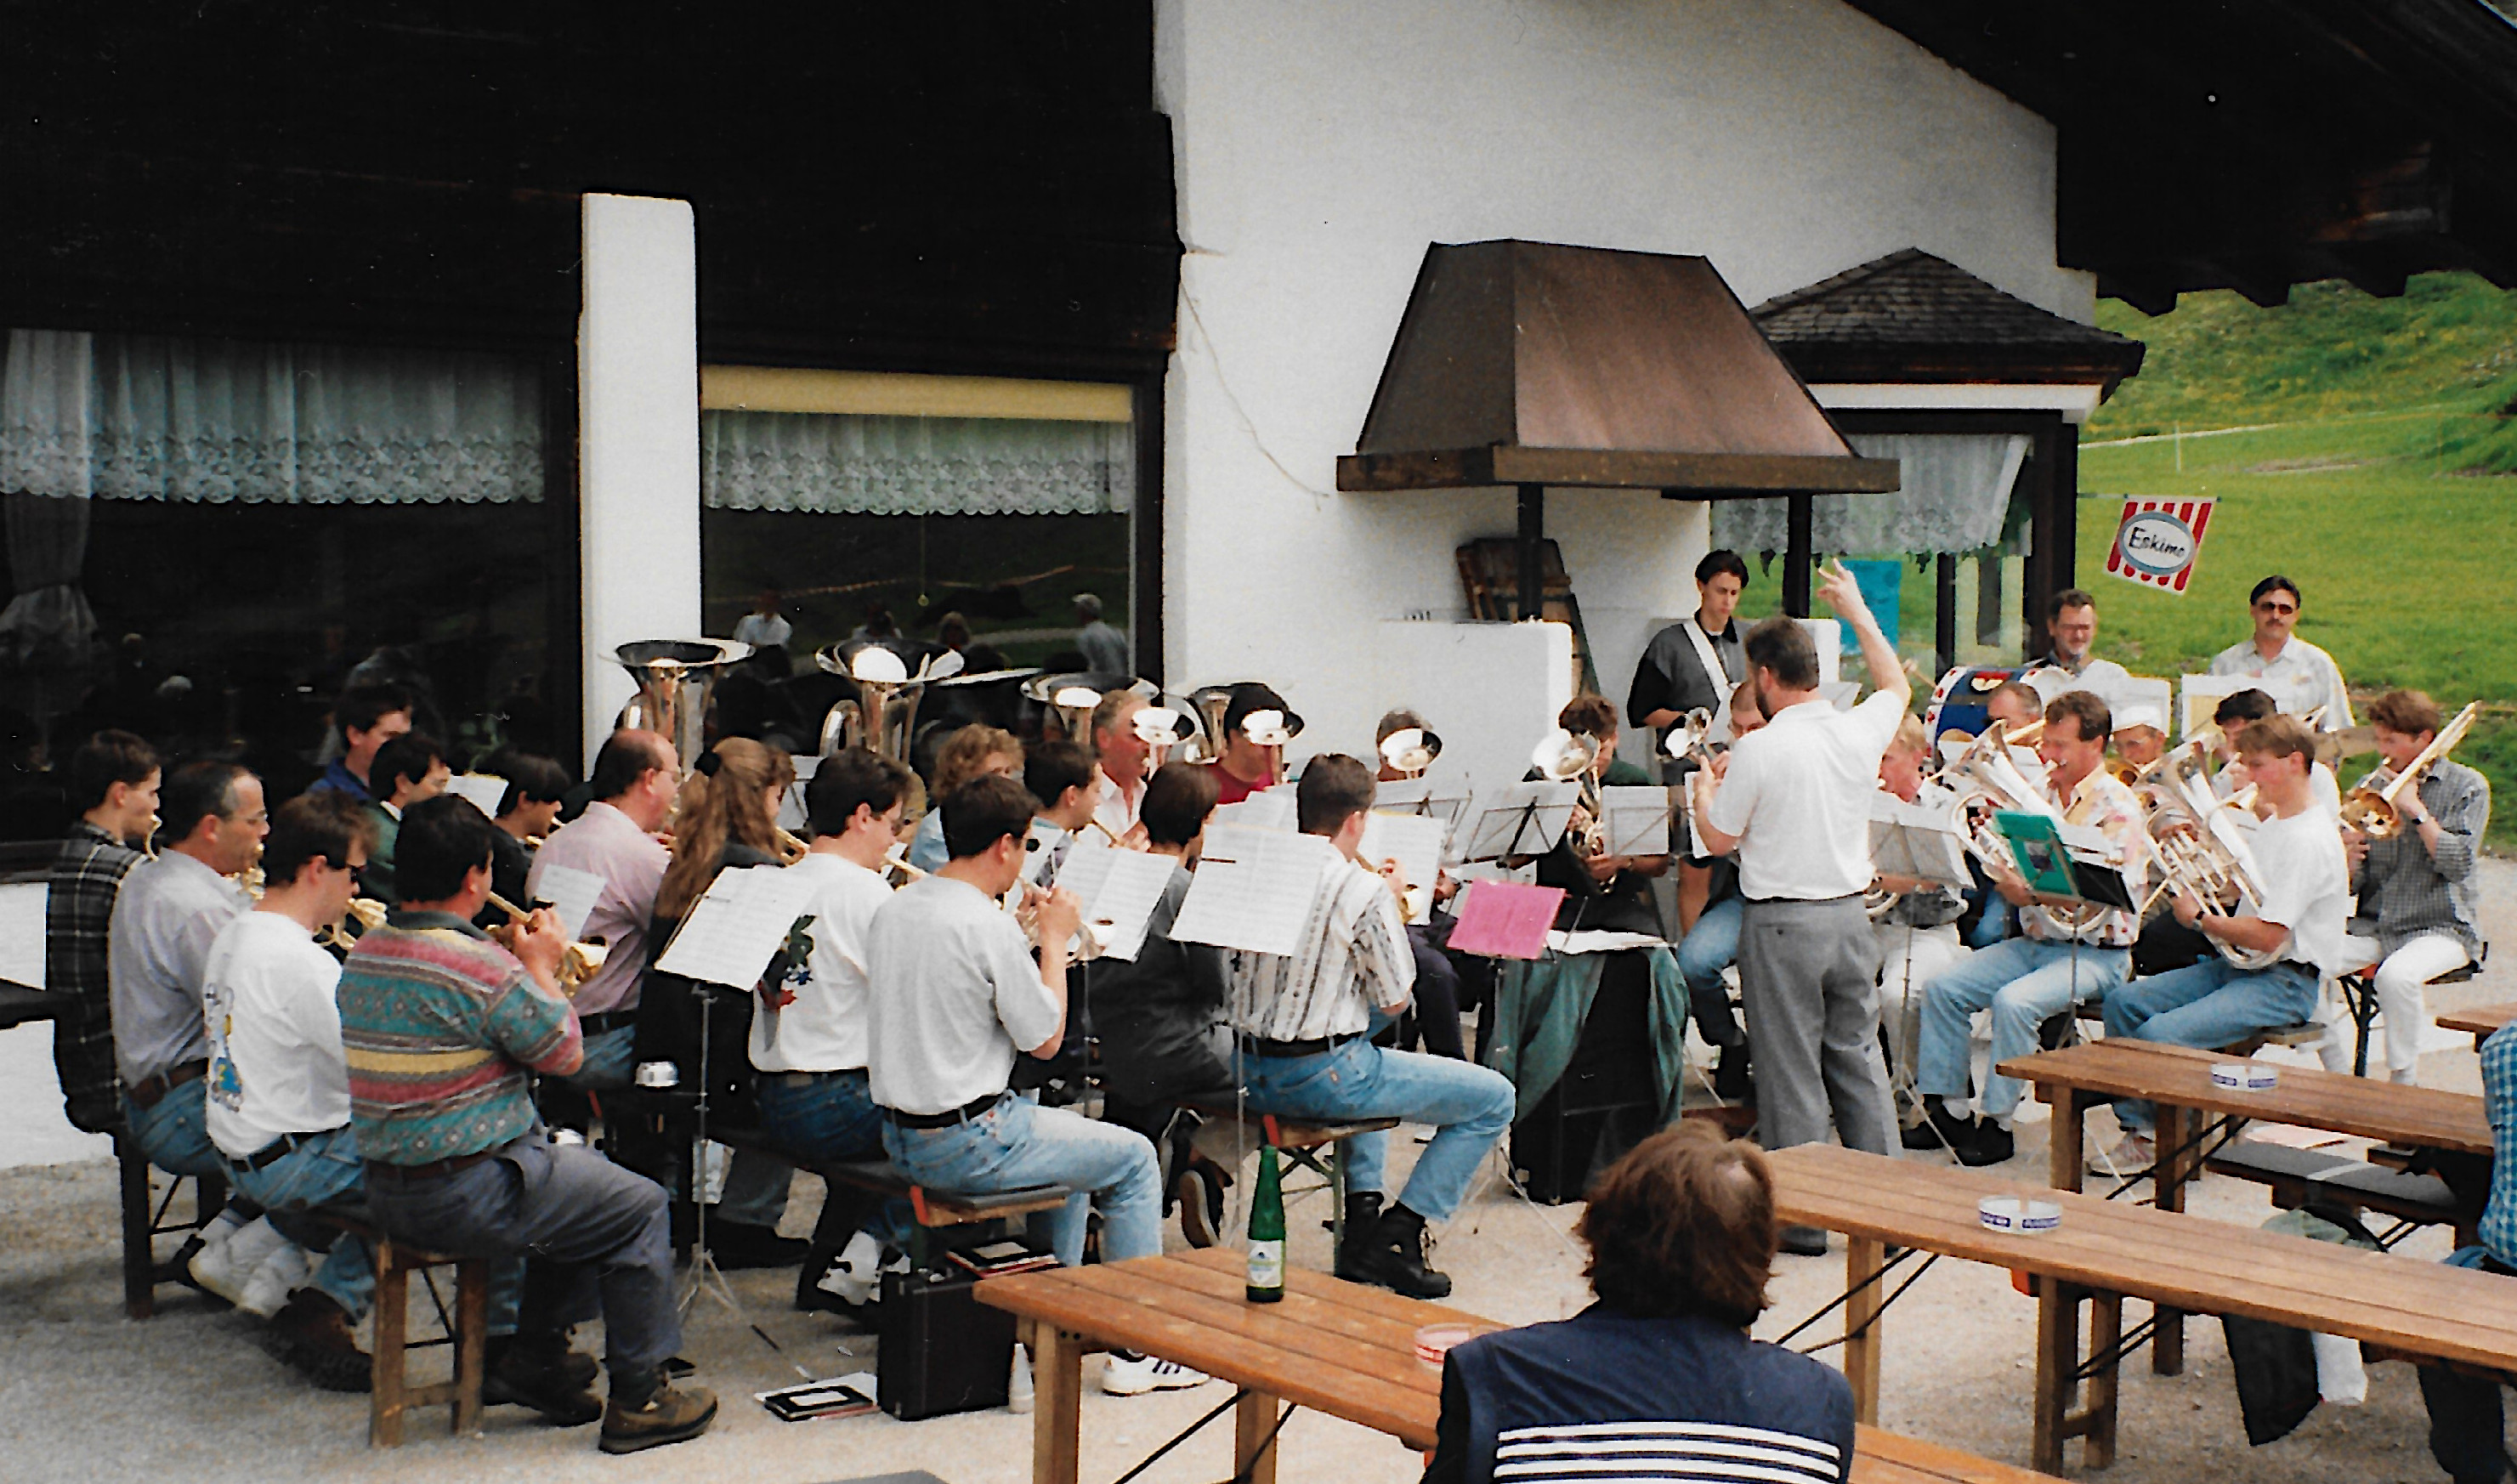
\includegraphics[width=0.93\linewidth]{./chap/1975-2000/1997/MGH-Ausflug-Seefeld-1997-1.jpg}
        \captionof{figure}{Frühschoppenkonzert beim Rest. Rosshütte}
    \end{MulticolFigure}

    Der Samstag war geprägt von musikalischen Aktivitäten; am Vormittag gab die
    Musikgesellschaft ein Frühschoppenkonzert im Restaurant Rosshütte, zu dem
    sie mit der Standseilbahn hinauffuhren. Am Abend führte ein Marsch durch die
    Fussgängerzone zum Kurpark, wo unter der Leitung von Gastdirigent Josef Brun
    ein unterhaltsames Konzert abgehalten wurde. Ein Highlight war der Auftritt
    des Alphorntrios der Musikgesellschaft, das für musikalische Abwechslung
    sorgte. Nach dem Konzert zog es die meisten erneut in den Bräukeller, wo bei
    ausgelassener Stimmung bis in die späte Nacht gefeiert wurde, wobei die
    eigene 6er Musik spontan für Stimmung sorgte. Viele liessen den Abend
    schliesslich im Western Saloon ausklingen.

    \multicolphoto{./chap/1975-2000/1997/MGH-Ausflug-Seefeld-1997-2.jpg}

    Den Abschluss der Reise bildete der Sonntagsbrunch, nach dem wir die
    Heimreise über Landeck und den Arlbergpass antraten, um wieder in die
    Schweiz zurückzukehren.

    \begin{MulticolFigure}
        \centering
        \captionof{figure}{Musiktag Hergiswil 1998}
        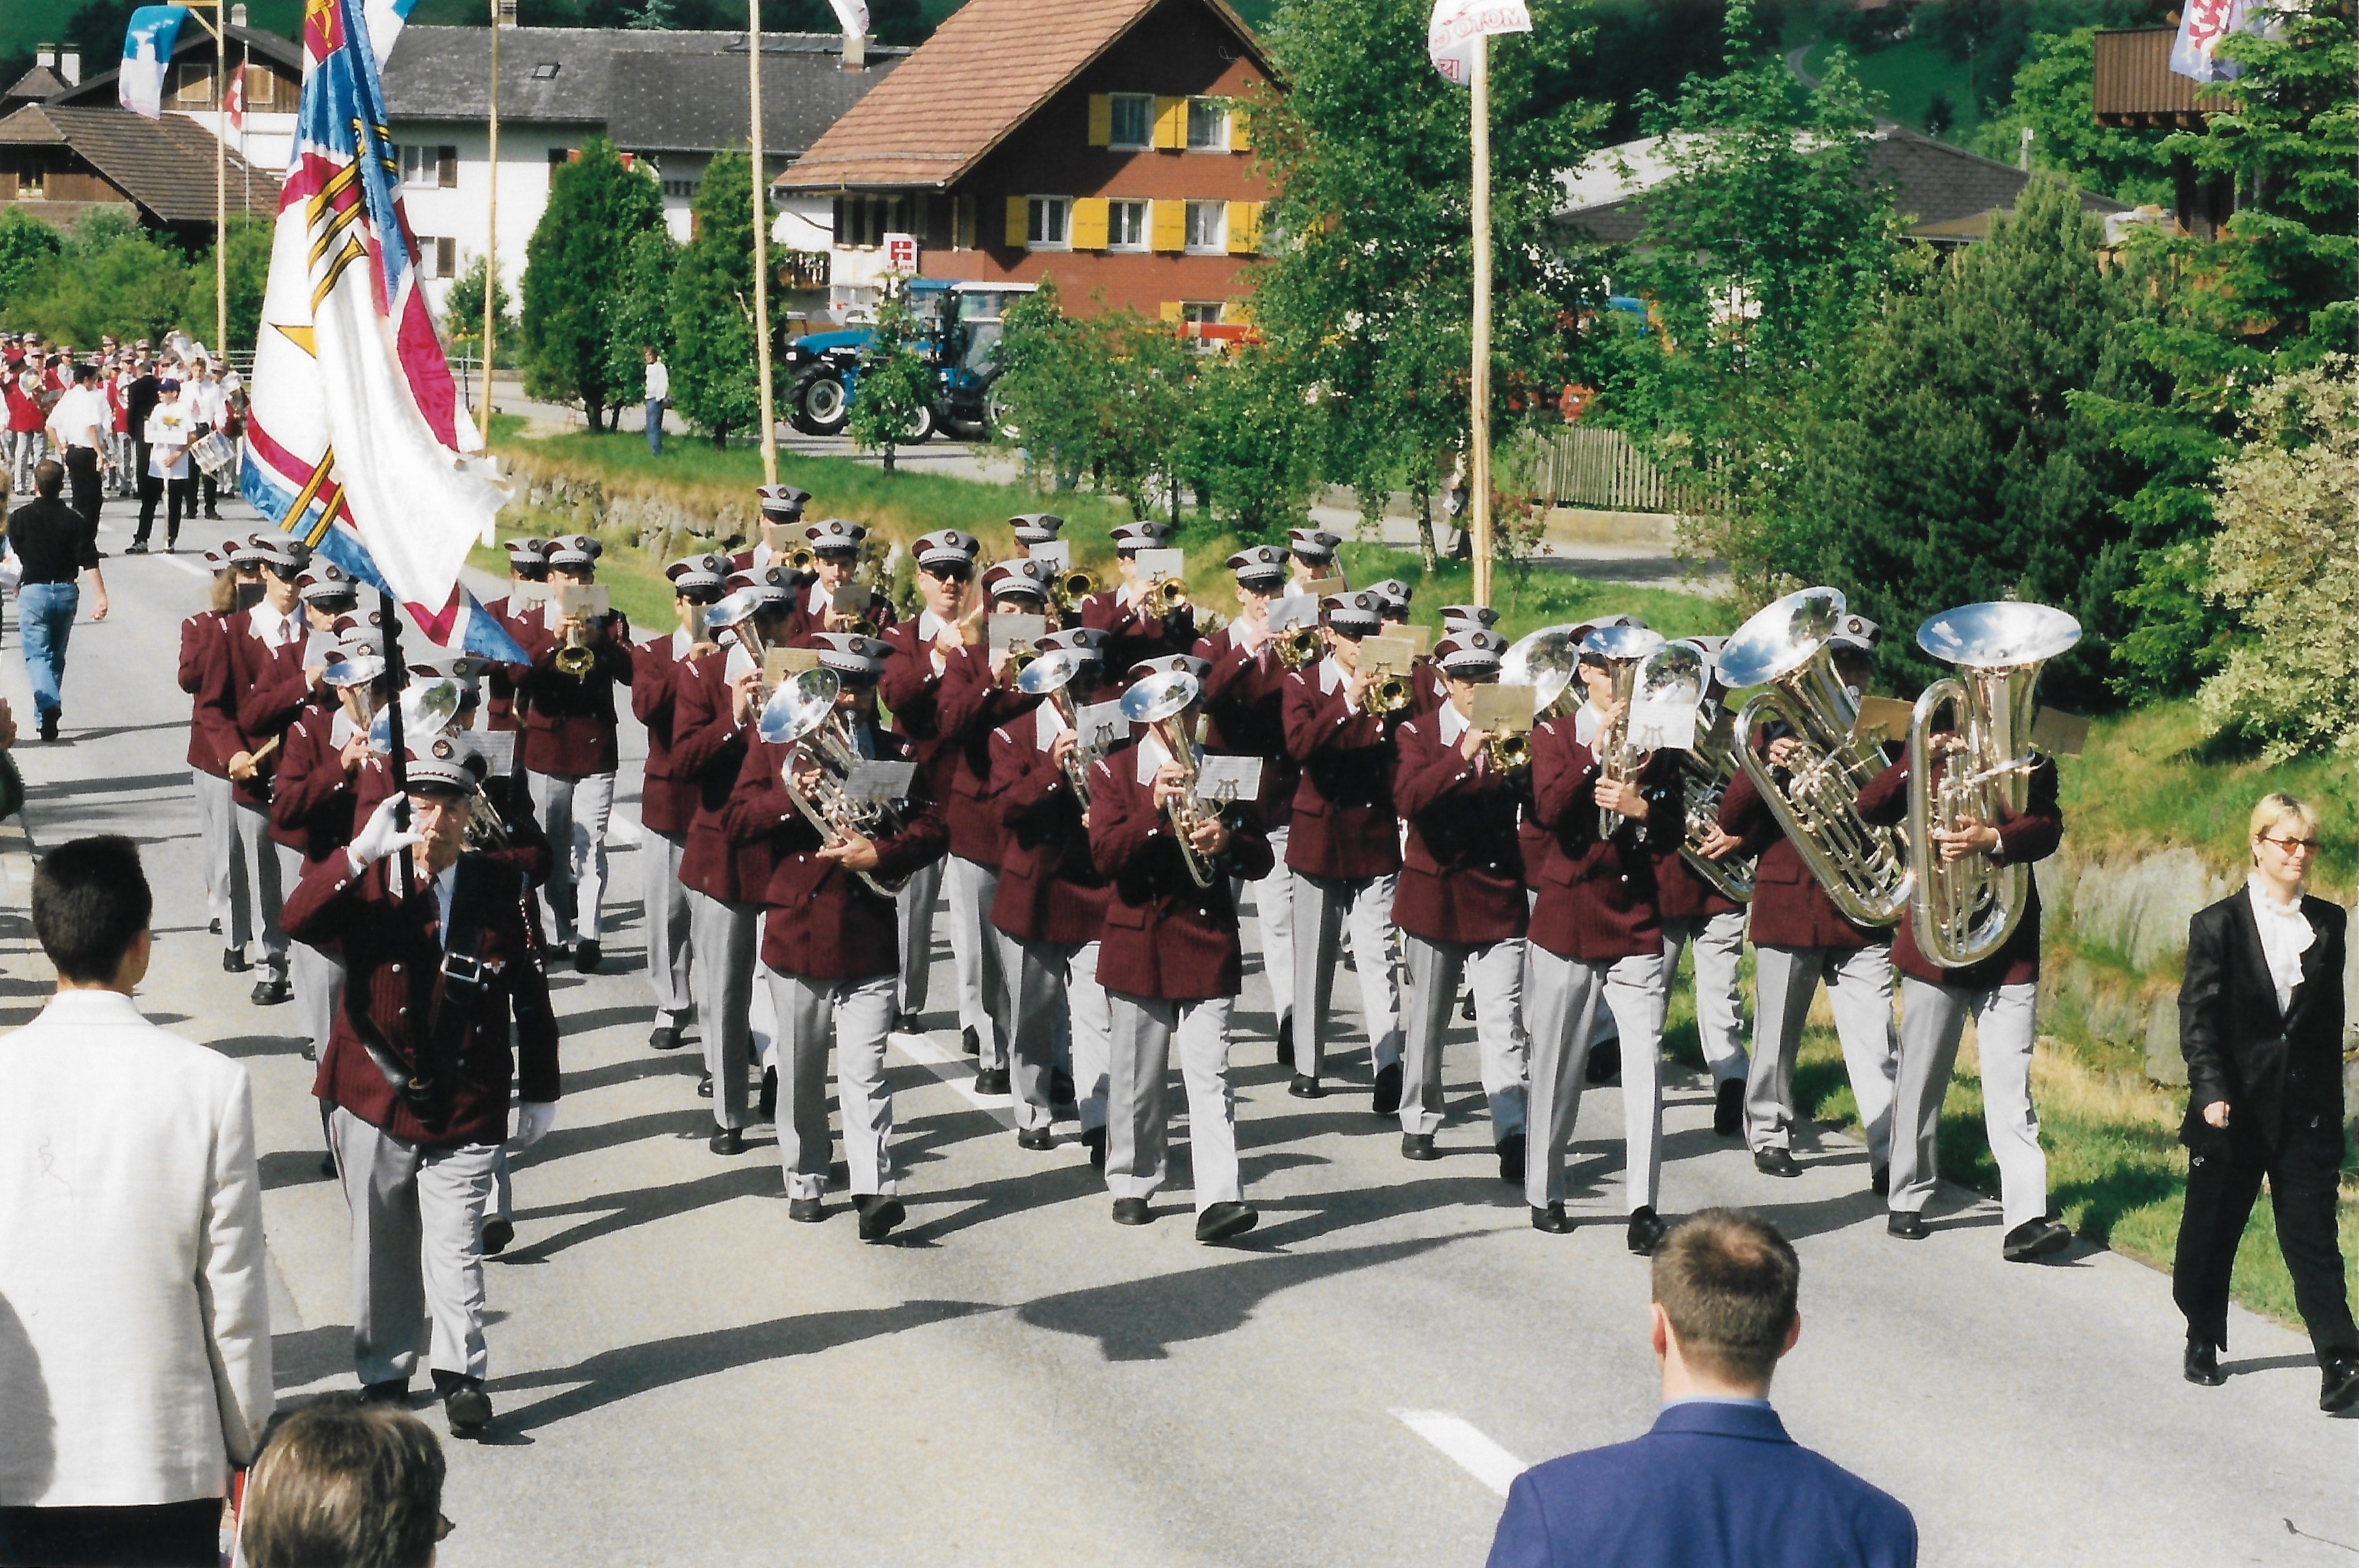
\includegraphics[width=0.85\linewidth]{./chap/1975-2000/1998/MGH-Musiktag-Hergiswil-1998.jpg}
    \end{MulticolFigure}

\end{history}

\groupphoto{0.93}{0.75}{./chap/1975-2000/1996/MGH-1996.jpg}
{\emph{Interlaken 1996}\\
    1. Reihe:\\
    Marcel Sennhauser, Alois Gassmann sen., Franz Estermann, Martin Estermann,
    Oskar Troxler, Albert Tschofen, Daniel Fleischli, Leo Estermann, Josef Wolf
    jun., Thomas Wolf, Franz Dörig\\
    2. Reihe:\\
    Reto Rüttimann, Alexander Troxler, Renate Burkhard, Anita Steiner, Beat
    Koller, Beat Bachmann, Peter Käppeli, Anton Bachmann, Jakob Estermann, Anton
    Kleemann, Guido Zurfluh\\
    3. Reihe:\\
    Karin Rüttimann, Armand Troxler, Othmar Estermann, Bruno Luterbach, Hermann
    Troxler, Christoph Troxler, Yvonne Emmenegger\\
    4. Reihe:\\
    Alois Gassmann jun., Hans Stöckli, Martin Troxler, Adrian Rüttimann, Werner
    Bucher, Bruno Estermann, Bruno Gretener, Kaspar Dörig, Jakob Suter\\
    5. Reihe:\\
    Pirmin Troxler, Beat Estermann, Franz Arnold, Martin Aregger, Stephan Wolf }
{fig:mgh-1996}


\begin{history}

    \subsubsection*{Prozession mit Schützenfahne 1999}
    Am Weissen Sonntag begleiteten wir die feierliche Prozession mit einem
    Marsch und gaben im Anschluss ein herzliches Ständchen. Doch dieser Tag wird
    uns vor allem wegen eines kleinen, unerwarteten Zwischenfalls in Erinnerung
    bleiben: Anstatt mit unserer eigenen Fahne stolz voranzuschreiten, fanden
    wir uns aus Versehen mit der Fahne der Feldschützen wieder, als wir durch
    das Dorf schritten. Diese heitere Verwechslung sorgte für Lächeln und
    amüsierte Gespräche unter den Anwesenden und bleibt ein charmantes Kapitel
    in unserer Geschichte.

    \begin{MulticolFigure}
        \centering
        \includegraphics[width=0.85\linewidth]{./chap/1975-2000/1999/MGH-mit-Schützenfahne.jpg}
        \captionof{figure}{MGH mit Schützenfahne}
    \end{MulticolFigure}

    \subsubsection*{Ausflug Südschwarzwald, 1999}

    Die Reise begann am Samstagmittag, als wir uns aufmachten, die malerische
    Region zu erkunden. Erster Halt war das Weingut von Andreas Neymeyer in
    Wettelbrunn, wo die MGH die Gelegenheit hatte, die köstlichen lokalen Weine
    zu probieren.

    % \multicolphoto{./chap/1975-2000/1999/MGH-Ausflug-Schwarzwald-1999.jpg}
    \begin{MulticolFigure}
        \centering
        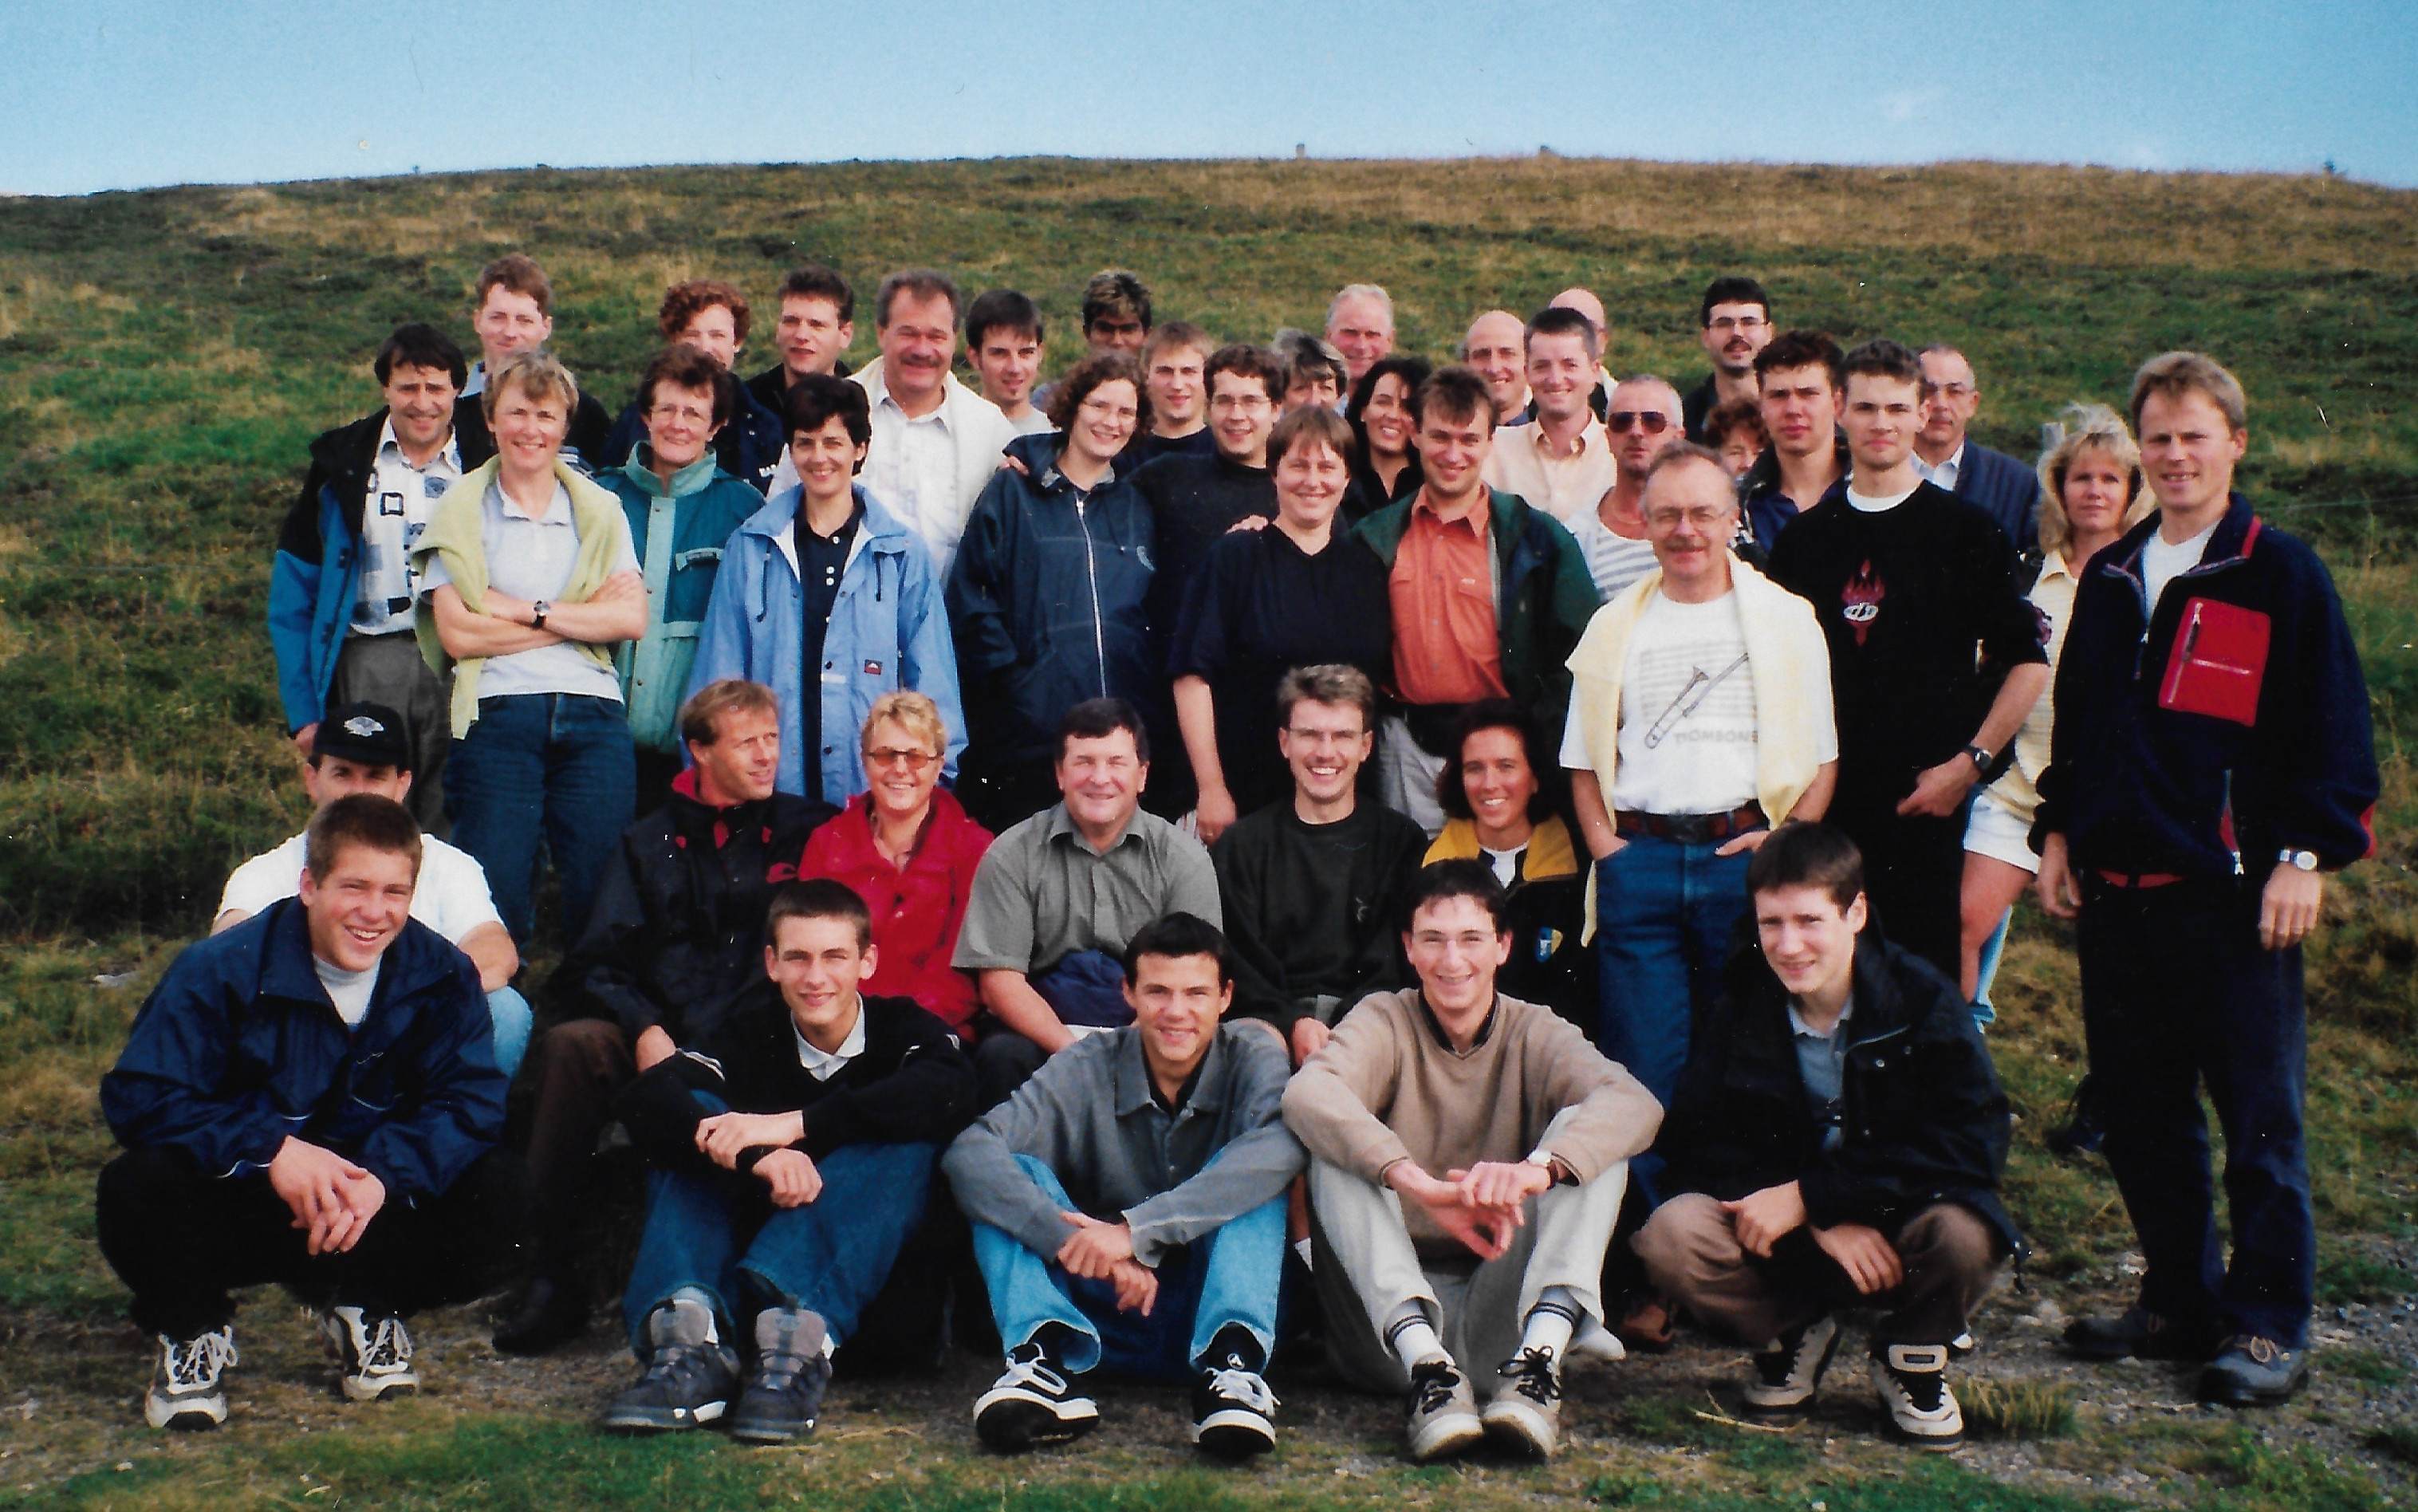
\includegraphics[width=0.9\linewidth]{./chap/1975-2000/1999/MGH-Ausflug-Schwarzwald-1999.jpg}
        \captionof{figure}{Ausflug in den Schwarzwald}
    \end{MulticolFigure}

    Anschliessend führte der Weg die Musikanten ins charmante Städtchen Staufen,
    wo sie einen Zwischenstopp einlegten, bevor sie dann den Abend im
    Jägerstüble verbrachten. Dort genossen sie ein ausgelassenes Beisammensein
    bei gutem Essen, Trank sowie Musik und Gesang, was den Gemeinschaftsgeist
    stärkte und für eine unvergessliche Atmosphäre sorgte. Die Übernachtung fand
    im gastlichen Haus Bergfried statt.

    Der Sonntag war von naturnahen Aktivitäten geprägt. Die Musikgesellschaft
    unternahm eine Wanderung zum Belchen, einem der höchsten Aussichtspunkte der
    Region, der mit seiner atemberaubenden Aussicht begeisterte. Danach stand
    ein Besuch der imposanten Klosterkirche in St. Blasien auf dem Programm, die
    mit ihrer architektonischen Schönheit beeindruckte.

    Die Rückfahrt nach Hildisrieden führte uns über Häusern und Waldhut nach
    Brugg und schloss damit ein Wochenende voller Erlebnisse.

    \subsubsection*{Neue Mehrzweckhalle Inpuls 1999/2000}

    Eine Bläsergruppe beteiligte sich an der feierlichen Einweihung des Zentrums
    Inpuls in der Silvesternacht, ein Moment, der die kulturelle Bedeutung des
    neuen Gemeinschaftszentrums für Hildisrieden unterstrich.

    Ein besonderer Meilenstein war dann die erste Konzertgelegenheit in der
    Mehrzweckhalle Inpuls. Diese neue Spielstätte erwies sich für die
    Musikgesellschaft als äusserst vorteilhaft. Sie bot nicht nur ausreichend
    Platz und praktische Annehmlichkeiten, sondern überzeugte auch durch ihre
    hervorragende Akustik, die die musikalischen Darbietungen wirkungsvoll zur
    Geltung brachte.

    Diese Ereignisse zu Beginn des Jahres 2000 markierten einen positiven Start
    in ein neues Jahrzehnt für die Musikgesellschaft Hildisrieden und
    verdeutlichten die wichtige Rolle der Musik und des kulturellen Engagements
    in der Gemeinde.

    \subsubsection*{Kant. Musikfest Kriens, 2000}

    Die Vorbereitungen begannen mit einem Konzert im Zentrum Inpuls am 11. Mai,
    bei dem neben der Musikgesellschaft Hildisrieden auch die MG Flühli und die
    Feldmusik Rothenburg auftraten. Dieses Konzert diente als erste Generalprobe
    für die Musikeranten, um sich auf das bevorstehende Fest einzustimmen.

    Eine weitere Gelegenheit, die Wettkampfstücke zu präsentieren und die Form
    zu testen, bot sich beim Gemeinschaftskonzert in Neuenkirch am 19. Mai. Hier
    teilte sich die Musikgesellschaft Hildisrieden die Bühne mit der Brass Band
    Harmonie Neuenkirch und der MG Romoos, was eine wertvolle Gelegenheit zum
    Austausch und zur Feinabstimmung bot.

    Der Höhepunkt dieser Vorbereitungen fand schliesslich am 27. Mai beim
    Kantonalmusikfest in Kriens statt. Trotz des strömenden Regens brachte die
    Musikgesellschaft, transportiert von der Auto AG Rothenburg, ihre
    musikalischen Darbietungen zur Aufführung: Das Aufgabestück \enquote{Focus}
    von Leon Vargas und das Selbstwahlstück \enquote{North-West Passage} von Roy
    Newsome. Beide Stücke wurden in unterschiedlichen Lokalitäten -- der Kirche
    und der Mehrzweckhalle -- vorgetragen, wobei die Musikerinnen und Musiker
    ihr Können unter Beweis stellten.

    Die Spannung löste sich bei der Rangverkündigung auf, doch die Ergebnisse
    entsprachen nicht den Hoffnungen der Musikgesellschaft Hildisrieden. Mit 155
    Punkten erreichte die MGH den 13. Platz von 14 teilnehmenden Vereinen in
    ihrer Klasse, was als enttäuschendes Resultat empfunden wurde. Im Bereich
    der Marschmusik konnte jedoch ein zufriedenstellender Mittelfeldplatz
    erzielt werden.

\end{history}





\groupphoto{0.93}{0.8}{./chap/1975-2000/2000/MGH-2000.jpg}
{\emph{Kriens 2000}\\
    1. Reihe:\\
    Josef Wolf, Christoph Erni, Franz Dörig, Pirmin Troxler, Dominik Wey, Armand
    Troxler, Urs Niederberger, Beat Estermann, Martin Estermann, Franz
    Estermann\\
    2. Reihe:\\
    Karin Rüttimann, Matthias Fellmann, Beat Bachmann, Renate Troxler, Kobi
    Banz, Angelika Wey, Stephan Wolf, Mathias Rub, Beat Koller\\
    3. Reihe:\\
    Christoph Troxler, Martin Troxler, Othmar Estermann, Adrian Rüttimann,
    Werner Bucher, Peter Käppeli, Anton Bachmann, Anton Kleemann\\
    4. Reihe:\\
    Dhani Bachmann, Andreas Thürig, Reto Rüttimann, Alexander Troxler, Hans
    Stöckli\\
    5. Reihe:\\
    Armin Schmid } {fig:mgh-2000}

